% !TeX spellcheck = nl_NL
\chapter{Data verwerving}

% inleiding van dit hoofdstuk, wat ga ik allemaal bespreken
In dit hoofdstuk wordt de verwerving van de data toegelicht. Er wordt eerst enkele belangrijke specificaties van de gebruikte toestellen besproken. Vervolgens worden de gehanteerde programma's doorgenomen op vlak van gebruikte data en type \gls{nn}. Het hoofdprogramma wordt in de Python-programmeertaal geschreven. Deze taal werd gekozen door de veelvuldige toepassingsmogelijkheden binnen \gls{ml}. Tot slot wordt de dataverwerving van de benchmark zelf ge\"illustreerd en besproken hoe de data opgeslagen wordt.

% Verkennen te gebruiken software
\section{Verkennen van software}
% in welke mate vertel ik hier al over pyrenn????
% uitleggen wat tensorflow is en hoe ik het gebruik. = tensorflowlite
% wat is er nodig om tf te laten runnen op gpu / of te controleren

% Verkennen devices
\section{Verkennen edge-devices}
	% welke benodigdheden zijn er om programma's te runnen; coral dev: tflite
	% aanvullende data zoals cpu% kost,...
	
% subsectie: structuur runV4
\section{Structuur programma}
In deze sectie wordt de structuur van het hoofdprogramma besproken. De belangrijkste onderdelen van de programma's worden toegelicht. Zo wordt er weergegeven hoe de verschillende \gls{nn}-modellen opgebouwd zijn en op welke data ze worden toegepast voor zowel het trainen als het uitvoeren. De benchmark bevat in totaal 10 verschillende subprogramma's. Elk van deze is een neuraal netwerk met een zekere complexiteit bedoeld voor weide variatie aan applicaties. Van de 10 subprogramma's kunnen er zes van gecategoriseerd worden als regressie en vier als classificatie. Voor elk subprogramma wordt er uitgelegd hoe het model wordt opgesteld, hoe het getraind wordt en hoe het uiteindelijk uitgevoerd wordt. Voor de benchmark is vooral het uitvoeren van de modellen van belang. Het opstellen en trainen van een \gls{nn} is een eenmalige taak en hoeft bijgevolg niet op edge-devices gebeuren.


	\subsection{Regressie subprogramma's}
	Voor de regressie subprogramma's werd er gekozen om gebruik te maken van pyrenn\footnote{Meer info over pyrenn is te vinden op https://pyrenn.readthedocs.io/en/latest/index.html}. Dit is een toolbox voor zowel Python als Matlab. Deze laat op een heel eenvoudige manier \gls{nn} trainen en uitvoeren. De pyrenn-toolbox heeft 2 dependencies of afhankelijkheden in Python. Deze zijn de gekende pandas en numpy packages.  De volgende subprogramma's worden opgesteld met behulp van de pyrenn-voorbeelden. 

		\subsubsection{Programma 1: compair}
		Het eerste subprogramma is een \textit{compressed air storage system} of een samengedrukte lucht opslagsysteem. Het systeem met drie verschillende inputs en 2 gewenste outputs. De praktische werking wordt verduidelijkt in figuur \ref{fig:compairPraktijk} maar wordt in deze thesis verder niet op in gegaan. Hier wordt er een \gls{rnn} toegepast. Dit is een regulier \gls{nn} waar er een terugkoppeling bestaat tussen een node naar een vorige laag toe. 
			
		\begin{figure}
			\centering
			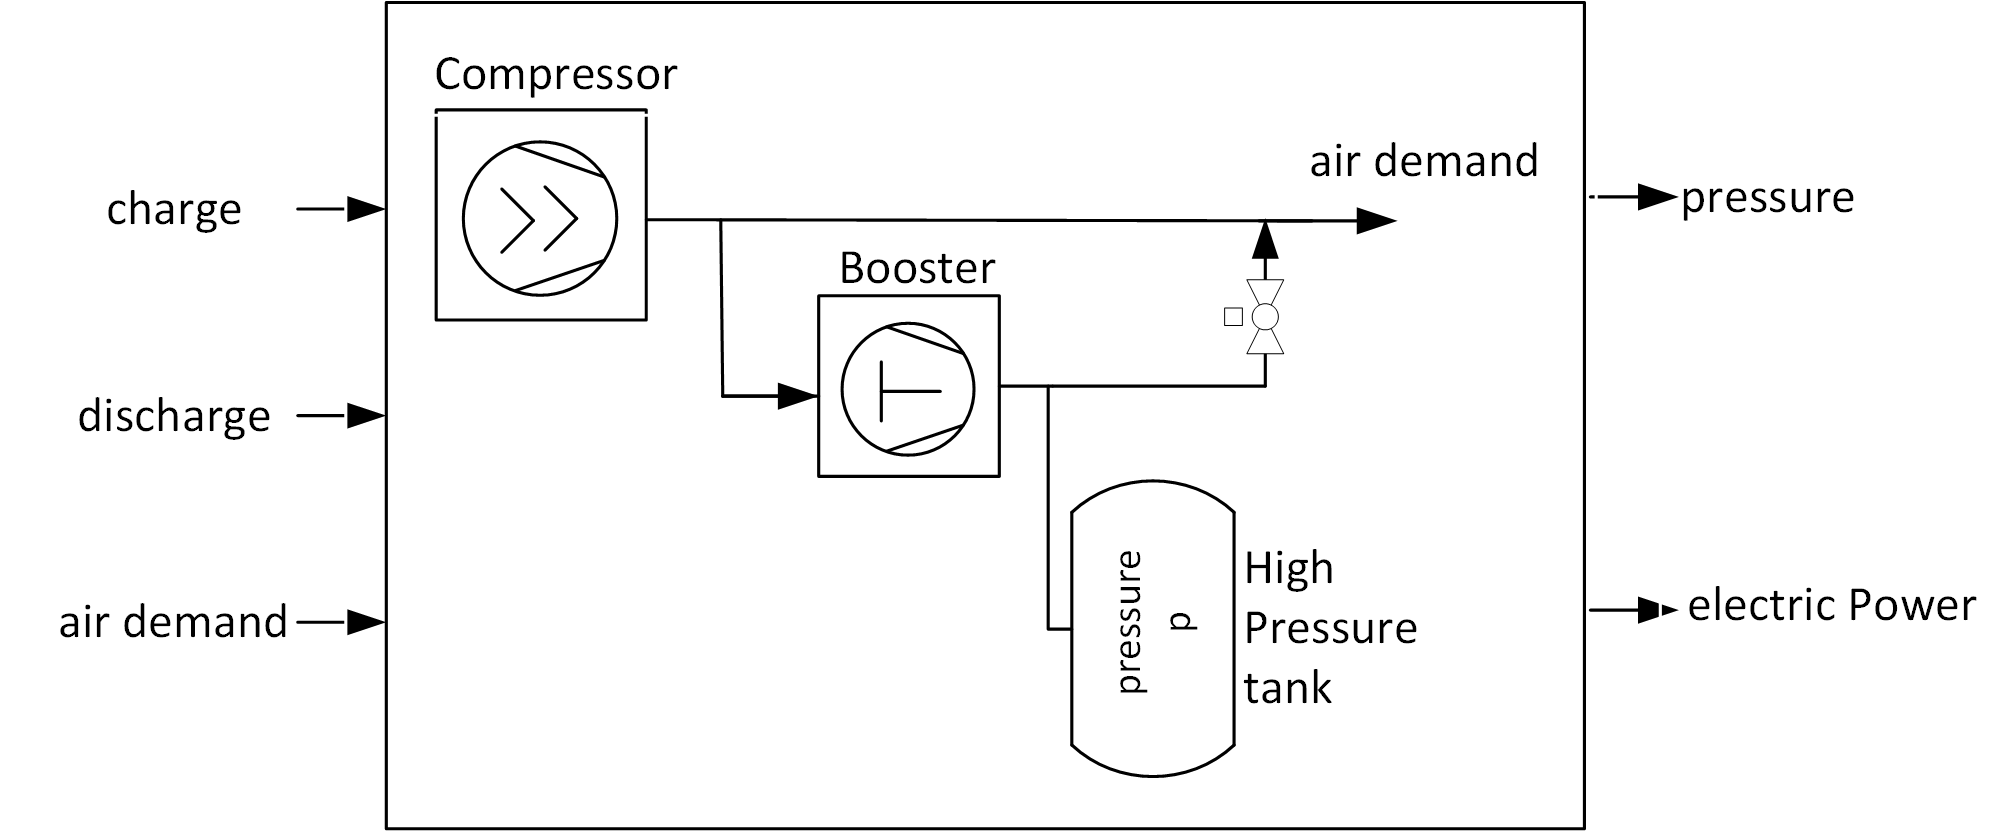
\includegraphics[width=120mm]{afbeeldingen/compairPraktijk.PNG}
			\caption{Praktische betekenis van het compair-subprogramma. \\Afbeelding te vinden op https://pyrenn.readthedocs.io/en/latest/examples.html\\ Website werd geraadpleegd op 10/04/2020.}
			\label{fig:compairPraktijk}
			%bron: https://medium.com/machine-learning-bites/machine-learning-decision-tree-classifier-9eb67cad263e
		\end{figure}
	
		\begin{table}[]
			\centering
			\begin{tabular}{ccccccc}
				\hline
				subprogramma                   & index & P1       & P2 & P3  & Y1       & Y2  \\ \hline
				\multicolumn{1}{c|}{compair}   & 464   & 0        & 1  & 0.8 & 7        & 8.4 \\
				\multicolumn{1}{c|}{friction}  & 14    & -3       &    &     & -0,29148 &     \\
				\multicolumn{1}{c|}{narendra4} & 80    & -0,54404 &    &     & -0,45803 &     \\
				\multicolumn{1}{c|}{pt2}       & 208   & -7,96923 &    &     & -0,44761 &     \\ \hline
			\end{tabular}
			\caption{Voorbeelden van de gebruikte data voor regressiemodellen.}
			\label{tab:dataVoorbeelden}
		\end{table}
	
			\paragraph{Aanmaken en trainen model}
			Voor dit subprogramma werd er gewerkt met een dataset voorzien door Pyrenn zelf. Deze dataset levert in totaal 960 data inzendingen voor de inputs en outputs. Hiervan zijn er 480 inzendingen voorzien voor trainen en 480 voor testen van het model. In tabel \ref{tab:dataVoorbeelden} kan u een voorbeeld vinden van \'e\'en datalijn. Hierbij is de inputdata $P$ een lijst van drie features $P1$, $P2$ en $P3$. Analoog geldt dat de te verwachten outputdata $Y$ een lijst voorstelt met twee features $Y1$ en $Y2$. Het \gls{nn} wordt hier gedefinieerd door vier lagen. Een inputlaag, twee verborgen lagen en een outputlaag. Het aantal nodes voor de input- en outputlaag zijn gekend: drie en twee nodes respectievelijk. Voor de twee hidden layers werd er gekozen om vijf nodes elk te implementeren.
			Het model kan gecre\"eerd worden met het commando \textit{CreateNN()} zoals te zien is in listing \ref{lst:codecreatemodel}. De variabele \textit{net} bevat de vorm van het model. In het commando kunnen parameters toegevoegd worden. Zo wordt in een lijst de grootte en de lengte van de laag meegegeven. De parameters $dIn$, $dIntern$ en $dOut$ kunnen gebruikt worden om wederkerende verbindingen te maken. Zo wordt in dit subprogramma dOut op de waarde 1 gezet om van de outputlaag een verbinding met een vertraging van 1 tijdsperiode naar de vorige laag aanbrengen. Vervolgens wordt het model getraind met de data met het commando \textit{train\_LM()}. Hierbij worden parameters zoals $k\_max$ en $E\_stop$ toegepast om respectievelijk aan te duiden voor hoeveel iteraties er maximaal getraind mag worden en de minimale fout dat bereikt mag worden. Tot slot word het model ook opgeslagen in een \gls{csv}-bestand via het commando \textit{saveNN()}. Het uitvoeren van het model kan dan op een apart device gebeuren. 

			\begin{lstlisting}[caption={Cre\"eren en trainen van pyrenn-model.},captionpos=b, label = {lst:codecreatemodel}]
	# Create and train NN
	net = pyrenn.CreateNN([3, 5, 5, 2], dIn=[0], dIntern=[], dOut=[1])
	net = pyrenn.train_LM(P, Y, net, verbose=True, k_max=500, E_stop=1e-5)
	# Save outputs to certain file
	prn.saveNN(net, "./models/compair.csv")
			\end{lstlisting}
			
			\paragraph{Uitvoeren model} 
			Via het commando \textit{loadNN()} kan het model van uit een bestand terug in een variabele worden opgeslagen. Het uitvoeren van het model zelf op testdata kan gebeuren via de instructie \textit{NNOut()}. Het resultaat hiervan wordt in de variabele $y$ opgeslagen zoals in listing \ref{lst:coderunmodel}. In vele toepassingen is het wenselijk dat variabele $y$ zo nauw mogelijk aansluit met de echte waarden $Y$. In deze thesis is de accuraatheid van het model echter niet van belang. De parameters die hier onderzocht worden zijn onafhankelijk van de accuraatheid van het model. Deze wordt dus ook niet berekend en verder gebruikt. 
	\begin{lstlisting}[caption={uitvoeren van pyrenn-model.},captionpos=b, label = {lst:coderunmodel}]
	# Load saved NN from file
	net = prn.loadNN("./models/compair.csv")
	# Calculate outputs of the trained NN for train and test data	
	y = prn.NNOut(P, net)
	\end{lstlisting}
		
		\subsubsection{Programma 2: friction}
		Het friction-subprogramma is een voorbeeld dat een fysische grootheid berekend. Het gaat hier over de wrijvingskracht $F$ in functie van de snelheid $v$. Deze grootheden voldoen aan formule \ref{eq:friction}. 
		\begin{equation}\label{eq:friction}
					F = \frac{\tanh(25 \cdot v)- \tanh(v)}{2} + \frac{\tanh(v)}{5}+0.03\cdot v			
		\end{equation}
		Uit deze formule kan er afgeleid worden dat we met statisch systeem met \'e\'en input, $v$, en \'e\'en output, $F$n werken. Voor analogie met de andere pyrenn-subprogramma's worden deze respectievelijk $P$ en $Y$ genoemd. De pyrenn-dataset waar we hier van gebruik maken bestaat 41 datapunten voor het trainen en 201 datapunten voor het testen van het model. Een voorbeeld van een datapunt kan in tabel \ref{tab:dataVoorbeelden} gevonden worden. Het model dat hier gebruikt wordt is een regulier \gls{nn} en bestaat uit vier lagen. De input- en outputlaag bestaan uit \'e\'en node. De twee hidden layers bestaan hier elk uit 3 nodes. Zowel het cre\"eren en trainen als het uitvoeren van het model gebeuren aan analoge wijze als in listing \ref{lst:codecreatemodel} en \ref{lst:coderunmodel}.
						
		\subsubsection{Programma 3: narendra4}
		Narendra4 is een programma dat de narendra4-functie\cite{narendra4} beschrijft. Dit is een voorbeeld van een dynamisch systeem met slechts \'e\'en output en \'e\'en input met vertraging en wordt beschreven in vergelijking \ref{eq:narendra4}. Een datapunt kan gevonden worden in tabel \ref{tab:dataVoorbeelden}. Het model zal ook een \gls{rnn} vormen. Hier zullen er grotere terugkoppelingen aanwezig zijn. Om een output $y_{k+1}$ te berekenen moeten de twee vorige inputs $p_{k-1}$ en $p_{k}$ ook bekend zijn. Er zal dus een vertraging van twee tijdsperiodes aanwezig zijn voor de inputnode. Dit vertaalt zich in de inputvariabele $dIn$ uit listing \ref{lst:narendra4} die nu gelijk is aan de waarde $[1,2]$. Op analoge wijze zijn er drie tijdsperiodes vertraging aanwezig voor de outputnode: $dOut$ is nu gelijk aan de waarde $[1,2,3]$. De twee tussenliggende verborgen lagen, die elk uit drie nodes bestaan, ondervinden zelf geen vertragingen. Het uitvoeren van het \gls{rnn} gebeurt weer op analoge wijze als in listing \ref{lst:coderunmodel}.
		
		\begin{equation}\label{eq:narendra4}
			y_{k+1} =\frac{ y_k \cdot y_{k-1} \cdot y_{k-2}\cdot p_{k-1}\cdot(y_{k-2}-1	)+ p_k} {1+(y_{k-1})^2+(y_{k-2})^2}	
		\end{equation}
		
		\begin{lstlisting}[caption={Cre\"eren en trainen van pyrenn-model voor narendra4.}, captionpos=b,label={lst:narendra4}]
	# Create and train NN
	net = pyrenn.CreateNN([1, 3, 3, 1], dIn=[1, 2], dIntern=[], dOut=[1, 2, 3])
	net = pyrenn.train_LM(P, Y, net, verbose=True, k_max=200, E_stop=1e-3)
	# Save outputs to certain file
	prn.saveNN(net, "./models/narendra4.csv")
		\end{lstlisting}
		
		\subsubsection{Programma 4: pt2}
		Het subprogramma pt2 is een programma dat een dynamisch systeem met \'e\'en input en \'e\'en output beschrijft. Het te gebruiken systeem hier is een tweede order transfer functie zoals in vergelijking \ref{eq:pt2} is opgetekend. De gebruikte pyrenn-dataset is ook hier een set met \'e\'en input feature, $P$, en \'e\'en output feature, $Y$. Ook van deze set is een datapunt opgenomen in tabel \ref{tab:dataVoorbeelden}. In totaal zijn er 1000 datapunten beschikbaar, waarvan 500 voor het trainen en 500 voor het testen. Voor het cre\"eren van dit model is er voor gekozen om naast de input- en outputlaag, twee hidden layers te implementeren met elk twee nodes. Voor deze hidden layers wordt er een vertraging van 1 tijdsperiode voorzien. Voor de uitgang wordt er een terugkoppeling van \'e\'en en twee tijdsperiodes voorzien? De waardes voor $dIntern$ en $dOut$ zijn dus respectievelijk $[1]$ en $[1,2]$ bij het aanmaken van dit model. Zowel trainen er runnen gebeuren analoog aan listing  \ref{lst:codecreatemodel} en \ref{lst:coderunmodel}.
		
		\begin{equation}\label{eq:pt2}
			G(s)= \frac{Y(s)}{U(s)} = \frac{10}{0.1 \cdot s^2 + s + 100}	
		\end{equation}
		
		\subsubsection{Programma 5: P0Y0-narendra4}
		Het P0Y0-narendra4-subprogramma is een programma dat gebruik maakt van al gekende data bij het uitvoeren van een getraind netwerk. Bij een \gls{rnn} is dit een interessant gegeven voor het model. Het kan meteen de vertraagde inputs and outputs een waarde geven in plaats van deze te initialiseren op nul. Dit bevordert de accuraatheid bij de start van het uitvoeren. Dit programma wordt toegepast op de narendra4-dataset. Het wordt dus op dezelfde wijze gecre\"eerd en getraind. Het verschil ligt bij het uitvoeren van het model. Hierbij worden er aan het $NNOut()$ commando drie willekeurig opeenvolgende datapunten in lijstvorm voor zowel de input als output. 

		\subsubsection{Programma 6: gradient}
		Dit subprogramma berekent de gradi\"ent-vector van de fout-marge van een \gls{nn}. Deze berekening is mogelijk met twee verschillende algoritmen gebeuren: \gls{rtrl} en \gls{bptt}. In deze thesis wordt er gebruik gemaakt van het \gls{rtrl}-algoritme. Deze werd in de documentatie beschrijven als een snellere oplossing bij het uitvoeren van het model. Dit subprogramma wordt toegepast op de pt2-dataset. Het model wordt bijgevolg op dezelfde wijze gedeclareerd als het pt2-subprogramma. De train- en run-commando's zijn te vinden in listing .

	\begin{lstlisting}[caption={Cre\"eren en trainen van pyrenn-model voor narendra4.}, captionpos=b,label={lst:narendra4}]
	# Create and train NN
	net = prn.CreateNN([1, 2, 2, 1], dIn=[0], dIntern=[1], dOut=[1, 2])
	data, net = prn.prepare_data(P, Y, net)
	# Run NN
	J, E, e = prn.RTRL(net, data)
	\end{lstlisting}
	

	\subsection{Classificatie subprogramma's}
		% verwerving data verscheidene programmas'
		% uitleg elk programma
		% uitleg tensorflow en keras
		
		\subsubsection{Programma 7: FashionMNIST}
		Het FashionMNIST-subprogramma is samen met NumberMNIST een van de klassiekers voor starters die kennis met \gls{ml} en \gls{nn} willen maken. Bovendien worden beide programma's ook regelmatig in andere benchmarks gebruikt wat vergelijkbaarheid bevordert. Voor deze redenen zullen we beiden ook in de benchmark opnemen. FashionMNIST is een \gls{nn} dat foto's van kledij-stukken probeert te classificeren volgens tien mogelijke labels. 
		
			\paragraph{Aanmaken en trainen model}
			
			% gebruik tensorflow en keras toevoegen
			
			Voor we het model beschrijven wordt er eerst de te gebruiken data verkent. De dataset\footnote{Datasets te vinden op: https://www.kaggle.com/zalando-research/fashionmnist, website geraadpleegd op 13/04/20.} van foto's en labels die voor het trainen gebruikt wordt, bestaat uit 60.000 instanties. Elke instantie uit de foto-dataset omvat een foto van 28 bij 28 pixels. Elke pixel bestaat hier uit 1 waarde en is dus geen RGB-pixel met drie waardes. In figuur \ref{fig:FashionMNIST-kledij} zijn er enkele voorbeelden van instanties terug te vinden. Voor het model opgesteld kan worden moet de data eerst nog verwerkt worden naar een schaal die voor de compiler van het model beter te verwerken is. De waarde van 1 pixel varieert tussen nul en 255. De waarden worden door het maximum, 255, gedeeld zodat deze tussen 0 en 1 komen te liggen. Vervolgens kan het model gedeclareerd worden. In listing \ref{lst:FashionMNISTtrain} wordt de declaratie, compilatie en het trainen van het model getoond. Het model bestaat uit drie lagen. Aan de inputlaag wordt de verwerkte data ingegeven in matrixvorm. Vervolgens worden de 784 waarden omgezet via een hidden layer met 128 nodes en een relu-activatiefunctie naar de output. In de outputlaag wordt er de $softmax$-activatiefunctie toegepast. Deze functie zorgt voor probabilistische uitkomst voor elke outputnode. Elke node zal hierdoor een waarde krijgen die overeenstemt met de kans dat het model de input acht overeen te komen met een bepaald label. De som van de waarden in alle outputnodes moet gelijk zijn aan 1. Na het declareren, wordt het model gecompileerd. In het $compile()$-commando worden verschillende parameters zoals optimizer en loss-functie meegedeeld aan de compiler. Deze bepalen de wijze waarop het model gecompileerd wordt. Tot slot wordt met het $fit()$-commando het trainen gestart. Hier worden de verwerkte inputdata en bijhorende labels aan toegevoegd.  
			
			
			\begin{figure}
				\centering
				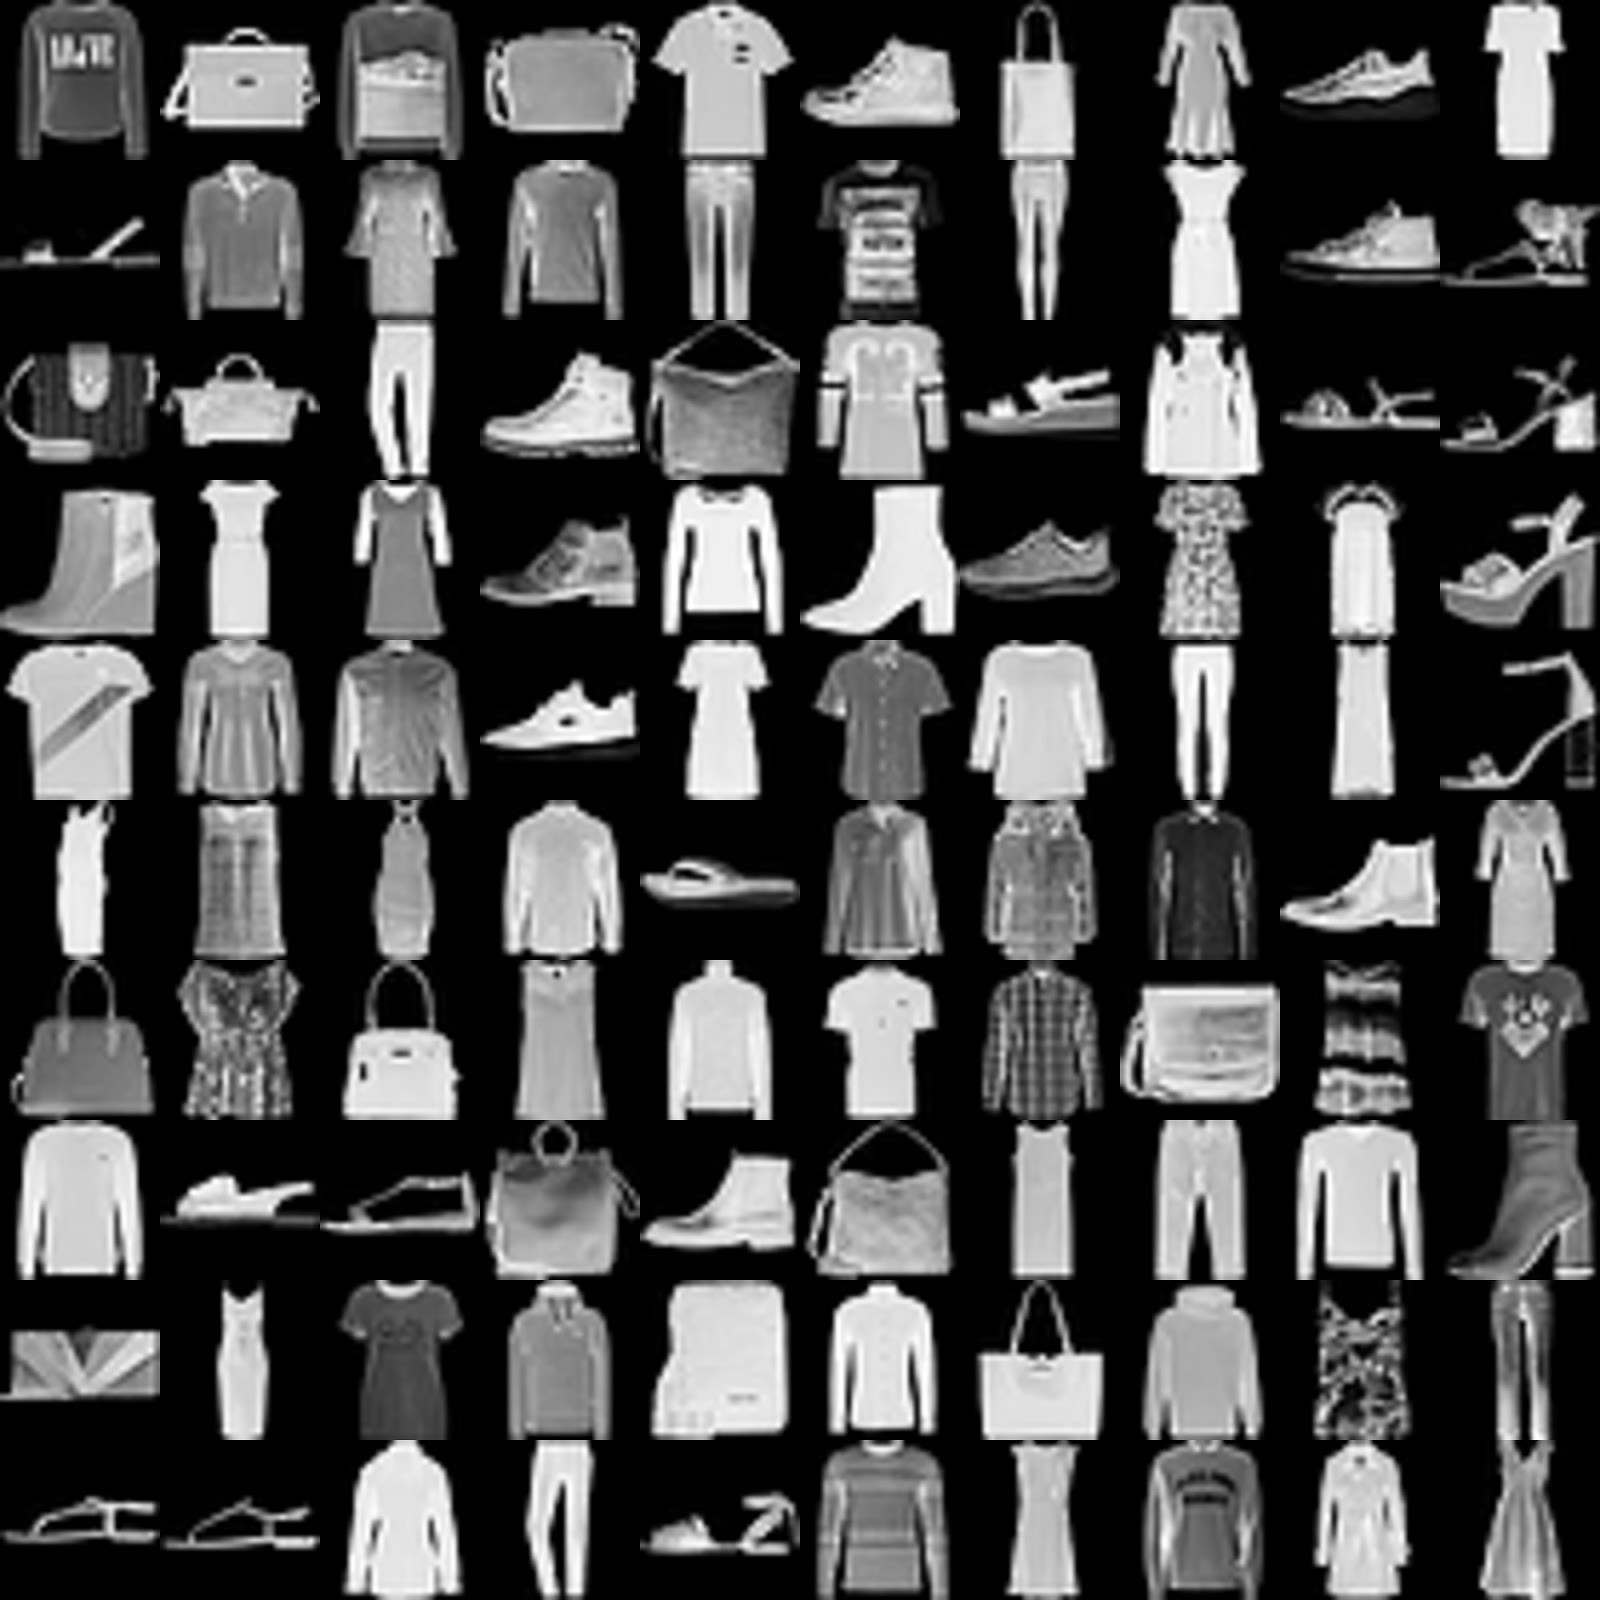
\includegraphics[width=80mm]{afbeeldingen/FashionMNIST_kledij.PNG}
				\caption{Enkele voorbeelden uit de FashionMNIST-dataset. \\Afbeelding te vinden op https://becominghuman.ai/how-to-create-a-clothing-classifier-fashion-mnist-program-on-google-colab-99f620c24fcd\\ Website werd geraadpleegd op 13/04/2020.}
				\label{fig:FashionMNIST-kledij}
				%bron: https://becominghuman.ai/how-to-create-a-clothing-classifier-fashion-mnist-program-on-google-colab-99f620c24fcd
			\end{figure}
	\begin{lstlisting}[caption={Cre\"eren en trainen van sequentieel model voor FashionMNIST.}, captionpos=b,label={lst:FashionMNISTtrain}]
	# Building the model
	model = tf.keras.Sequential([
		keras.layers.Flatten(input_shape=(28, 28)),
		keras.layers.Dense(128, activation="relu"),
		# the probability for each given class (total =1)
		keras.layers.Dense(10, activation="softmax")]) 
	# Compile the model
	model.compile(optimizer="adam",
		loss="sparse_categorical_crossentropy",
		metrics=["accuracy"])
	# training the model
	model.fit(train_images, train_labels, epochs=5)
	\end{lstlisting}			
			
		
			
			\paragraph{Uitvoeren model}
			
			

		\subsubsection{Programma 8: NumberMNIST}
		% waar gaat het programma in se over?
		% formule?
		% Data-structuut? grootte
		% aanmaken van model,
		% trainen van model
		% runnen van model
		\subsubsection{Programma 9: catsVSdogs}
		% waar gaat het programma in se over?
		% formule?
		% Data-structuut? grootte
		% aanmaken van model,
		% trainen van model
		% runnen van model
		\subsubsection{Programma 10: Image Recognition}
	% waar gaat het programma in se over?
		% formule?
		% Data-structuut? grootte
		% aanmaken van model,
		% trainen van model
		% runnen van model
	\subsection{Conversie naar TFLite}
		Doordat er in deze thesis gebruik gemaakt wordt van devices die met enkel \gls{tfl} werken worden de modellen omgezet naar een \gls{tfl}-model. Dit gebeurt door een convertor-object te cre\"eren van het bestaande keras-model. Op deze convertor worden optimalisatietechnieken uitgevoerd waarna het model wordt omgezet naar een \gls{tfl}-equivalent model. Dit model wordt vervolgens met het commando $write()$ uitgeschreven naar het gewenste bestand. Dit nieuwe model kan vervolgens opgeroepen worden voor uitvoering op gewenste momenten. In listing \ref{lst:TFLconversie} kan de gebruikte code terug gevonden worden.
	\begin{lstlisting}[caption={Converteren naar een \gls{tfl}-model.}, captionpos=b,label={lst:TFLconversie}]
	# Convert the model
	converter = tf.lite.TFLiteConverter.from_keras_model(model)
	converter.optimizations = [tf.lite.Optimize.DEFAULT]
	tflite_quant_model = converter.convert()
	# Saving tflite model
	open(path_model + "fashionMNISTmodel.tflite", "wb").write(tflite_quant_model)
	\end{lstlisting}	
% uitleggen ophalen data zoals cpu% en tijddata
\section{Uitvoeren metingen}


% Hoe opslaan data
\section{Opslaan van data}
	% gebruik maken van unieke filenaam